\documentclass[1p]{elsarticle_modified}
%\bibliographystyle{elsarticle-num}

%\usepackage[colorlinks]{hyperref}
%\usepackage{abbrmath_seonhwa} %\Abb, \Ascr, \Acal ,\Abf, \Afrak
\usepackage{amsfonts}
\usepackage{amssymb}
\usepackage{amsmath}
\usepackage{amsthm}
\usepackage{scalefnt}
\usepackage{amsbsy}
\usepackage{kotex}
\usepackage{caption}
\usepackage{subfig}
\usepackage{color}
\usepackage{graphicx}
\usepackage{xcolor} %% white, black, red, green, blue, cyan, magenta, yellow
\usepackage{float}
\usepackage{setspace}
\usepackage{hyperref}

\usepackage{tikz}
\usetikzlibrary{arrows}

\usepackage{multirow}
\usepackage{array} % fixed length table
\usepackage{hhline}

%%%%%%%%%%%%%%%%%%%%%
\makeatletter
\renewcommand*\env@matrix[1][\arraystretch]{%
	\edef\arraystretch{#1}%
	\hskip -\arraycolsep
	\let\@ifnextchar\new@ifnextchar
	\array{*\c@MaxMatrixCols c}}
\makeatother %https://tex.stackexchange.com/questions/14071/how-can-i-increase-the-line-spacing-in-a-matrix
%%%%%%%%%%%%%%%

\usepackage[normalem]{ulem}

\newcommand{\msout}[1]{\ifmmode\text{\sout{\ensuremath{#1}}}\else\sout{#1}\fi}
%SOURCE: \msout is \stkout macro in https://tex.stackexchange.com/questions/20609/strikeout-in-math-mode

\newcommand{\cancel}[1]{
	\ifmmode
	{\color{red}\msout{#1}}
	\else
	{\color{red}\sout{#1}}
	\fi
}

\newcommand{\add}[1]{
	{\color{blue}\uwave{#1}}
}

\newcommand{\replace}[2]{
	\ifmmode
	{\color{red}\msout{#1}}{\color{blue}\uwave{#2}}
	\else
	{\color{red}\sout{#1}}{\color{blue}\uwave{#2}}
	\fi
}

\newcommand{\Sol}{\mathcal{S}} %segment
\newcommand{\D}{D} %diagram
\newcommand{\A}{\mathcal{A}} %arc


%%%%%%%%%%%%%%%%%%%%%%%%%%%%%5 test

\def\sl{\operatorname{\textup{SL}}(2,\Cbb)}
\def\psl{\operatorname{\textup{PSL}}(2,\Cbb)}
\def\quan{\mkern 1mu \triangleright \mkern 1mu}

\theoremstyle{definition}
\newtheorem{thm}{Theorem}[section]
\newtheorem{prop}[thm]{Proposition}
\newtheorem{lem}[thm]{Lemma}
\newtheorem{ques}[thm]{Question}
\newtheorem{cor}[thm]{Corollary}
\newtheorem{defn}[thm]{Definition}
\newtheorem{exam}[thm]{Example}
\newtheorem{rmk}[thm]{Remark}
\newtheorem{alg}[thm]{Algorithm}

\newcommand{\I}{\sqrt{-1}}
\begin{document}

%\begin{frontmatter}
%
%\title{Boundary parabolic representations of knots up to 8 crossings}
%
%%% Group authors per affiliation:
%\author{Yunhi Cho} 
%\address{Department of Mathematics, University of Seoul, Seoul, Korea}
%\ead{yhcho@uos.ac.kr}
%
%
%\author{Seonhwa Kim} %\fnref{s_kim}}
%\address{Center for Geometry and Physics, Institute for Basic Science, Pohang, 37673, Korea}
%\ead{ryeona17@ibs.re.kr}
%
%\author{Hyuk Kim}
%\address{Department of Mathematical Sciences, Seoul National University, Seoul 08826, Korea}
%\ead{hyukkim@snu.ac.kr}
%
%\author{Seokbeom Yoon}
%\address{Department of Mathematical Sciences, Seoul National University, Seoul, 08826,  Korea}
%\ead{sbyoon15@snu.ac.kr}
%
%\begin{abstract}
%We find all boundary parabolic representation of knots up to 8 crossings.
%
%\end{abstract}
%\begin{keyword}
%    \MSC[2010] 57M25 
%\end{keyword}
%
%\end{frontmatter}

%\linenumbers
%\tableofcontents
%
\newcommand\colored[1]{\textcolor{white}{\rule[-0.35ex]{0.8em}{1.4ex}}\kern-0.8em\color{red} #1}%
%\newcommand\colored[1]{\textcolor{white}{ #1}\kern-2.17ex	\textcolor{white}{ #1}\kern-1.81ex	\textcolor{white}{ #1}\kern-2.15ex\color{red}#1	}

{\Large $\underline{12a_{0400}~(K12a_{0400})}$}

\setlength{\tabcolsep}{10pt}
\renewcommand{\arraystretch}{1.6}
\vspace{1cm}\begin{tabular}{m{100pt}>{\centering\arraybackslash}m{274pt}}
\multirow{5}{120pt}{
	\centering
	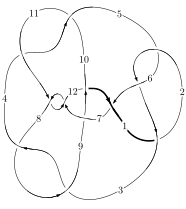
\includegraphics[width=112pt]{../../../GIT/diagram.site/Diagrams/png/1201_12a_0400.png}\\
\ \ \ A knot diagram\footnotemark}&
\allowdisplaybreaks
\textbf{Linearized knot diagam} \\
\cline{2-2}
 &
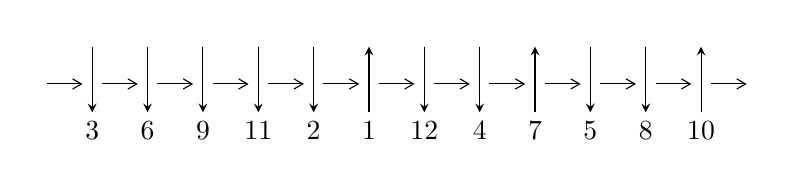
\begin{tikzpicture}[x=20pt, y=17pt]
	% nodes
	\node (C0) at (0, 0) {};
	\node (C1) at (1, 0) {};
	\node (C1U) at (1, +1) {};
	\node (C1D) at (1, -1) {3};

	\node (C2) at (2, 0) {};
	\node (C2U) at (2, +1) {};
	\node (C2D) at (2, -1) {6};

	\node (C3) at (3, 0) {};
	\node (C3U) at (3, +1) {};
	\node (C3D) at (3, -1) {9};

	\node (C4) at (4, 0) {};
	\node (C4U) at (4, +1) {};
	\node (C4D) at (4, -1) {11};

	\node (C5) at (5, 0) {};
	\node (C5U) at (5, +1) {};
	\node (C5D) at (5, -1) {2};

	\node (C6) at (6, 0) {};
	\node (C6U) at (6, +1) {};
	\node (C6D) at (6, -1) {1};

	\node (C7) at (7, 0) {};
	\node (C7U) at (7, +1) {};
	\node (C7D) at (7, -1) {12};

	\node (C8) at (8, 0) {};
	\node (C8U) at (8, +1) {};
	\node (C8D) at (8, -1) {4};

	\node (C9) at (9, 0) {};
	\node (C9U) at (9, +1) {};
	\node (C9D) at (9, -1) {7};

	\node (C10) at (10, 0) {};
	\node (C10U) at (10, +1) {};
	\node (C10D) at (10, -1) {5};

	\node (C11) at (11, 0) {};
	\node (C11U) at (11, +1) {};
	\node (C11D) at (11, -1) {8};

	\node (C12) at (12, 0) {};
	\node (C12U) at (12, +1) {};
	\node (C12D) at (12, -1) {10};
	\node (C13) at (13, 0) {};

	% arrows
	\draw[->,>={angle 60}]
	(C0) edge (C1) (C1) edge (C2) (C2) edge (C3) (C3) edge (C4) (C4) edge (C5) (C5) edge (C6) (C6) edge (C7) (C7) edge (C8) (C8) edge (C9) (C9) edge (C10) (C10) edge (C11) (C11) edge (C12) (C12) edge (C13) ;	\draw[->,>=stealth]
	(C1U) edge (C1D) (C2U) edge (C2D) (C3U) edge (C3D) (C4U) edge (C4D) (C5U) edge (C5D) (C6D) edge (C6U) (C7U) edge (C7D) (C8U) edge (C8D) (C9D) edge (C9U) (C10U) edge (C10D) (C11U) edge (C11D) (C12D) edge (C12U) ;
	\end{tikzpicture} \\
\hhline{~~} \\& 
\textbf{Solving Sequence} \\ \cline{2-2} 
 &
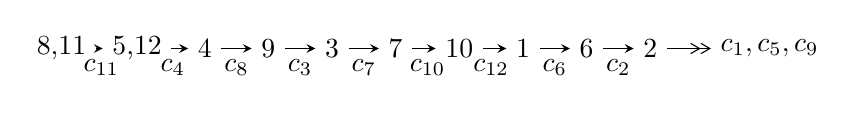
\begin{tikzpicture}[x=23pt, y=7pt]
	% node
	\node (A0) at (-1/8, 0) {8,11};
	\node (A1) at (17/16, 0) {5,12};
	\node (A2) at (17/8, 0) {4};
	\node (A3) at (25/8, 0) {9};
	\node (A4) at (33/8, 0) {3};
	\node (A5) at (41/8, 0) {7};
	\node (A6) at (49/8, 0) {10};
	\node (A7) at (57/8, 0) {1};
	\node (A8) at (65/8, 0) {6};
	\node (A9) at (73/8, 0) {2};
	\node (C1) at (1/2, -1) {$c_{11}$};
	\node (C2) at (13/8, -1) {$c_{4}$};
	\node (C3) at (21/8, -1) {$c_{8}$};
	\node (C4) at (29/8, -1) {$c_{3}$};
	\node (C5) at (37/8, -1) {$c_{7}$};
	\node (C6) at (45/8, -1) {$c_{10}$};
	\node (C7) at (53/8, -1) {$c_{12}$};
	\node (C8) at (61/8, -1) {$c_{6}$};
	\node (C9) at (69/8, -1) {$c_{2}$};
	\node (A10) at (11, 0) {$c_{1},c_{5},c_{9}$};

	% edge
	\draw[->,>=stealth]	
	(A0) edge (A1) (A1) edge (A2) (A2) edge (A3) (A3) edge (A4) (A4) edge (A5) (A5) edge (A6) (A6) edge (A7) (A7) edge (A8) (A8) edge (A9) ;
	\draw[->>,>={angle 60}]	
	(A9) edge (A10);
\end{tikzpicture} \\ 

\end{tabular} \\

\footnotetext{
The image of knot diagram is generated by the software ``\textbf{Draw programme}" developed by Andrew Bartholomew(\url{http://www.layer8.co.uk/maths/draw/index.htm\#Running-draw}), where we modified some parts for our purpose(\url{https://github.com/CATsTAILs/LinksPainter}).
}\phantom \\ \newline 
\centering \textbf{Ideals for irreducible components\footnotemark of $X_{\text{par}}$} 
 
\begin{align*}
I^u_{1}&=\langle 
26679 u^{42}+790144 u^{41}+\cdots+8192 b+610828288,\\
\phantom{I^u_{1}}&\phantom{= \langle  }10603 u^{42}+301637 u^{41}+\cdots+8192 a+19992576,\;u^{43}+30 u^{42}+\cdots+385024 u+16384\rangle \\
I^u_{2}&=\langle 
-8.60222\times10^{37} a^{27} u^{2}-3.77941\times10^{39} a^{26} u^{2}+\cdots-2.58200\times10^{42} a-7.32442\times10^{41},\\
\phantom{I^u_{2}}&\phantom{= \langle  }2 a^{27} u^2-7 a^{26} u^2+\cdots+3296 a+2157,\;u^3- u^2+2 u-1\rangle \\
I^u_{3}&=\langle 
-9 u^{25}+6 u^{24}+\cdots+b-9,\;18 u^{25}-24 u^{24}+\cdots+a+8,\;u^{26}- u^{25}+\cdots+u+1\rangle \\
\\
\end{align*}
\raggedright * 3 irreducible components of $\dim_{\mathbb{C}}=0$, with total 153 representations.\\
\footnotetext{All coefficients of polynomials are rational numbers. But the coefficients are sometimes approximated in decimal forms when there is not enough margin.}
\newpage
\renewcommand{\arraystretch}{1}
\centering \section*{I. $I^u_{1}= \langle 2.67\times10^{4} u^{42}+7.90\times10^{5} u^{41}+\cdots+8192 b+6.11\times10^{8},\;1.06\times10^{4} u^{42}+3.02\times10^{5} u^{41}+\cdots+8192 a+2.00\times10^{7},\;u^{43}+30 u^{42}+\cdots+385024 u+16384 \rangle$}
\flushleft \textbf{(i) Arc colorings}\\
\begin{tabular}{m{7pt} m{180pt} m{7pt} m{180pt} }
\flushright $a_{8}=$&$\begin{pmatrix}0\\u\end{pmatrix}$ \\
\flushright $a_{11}=$&$\begin{pmatrix}1\\0\end{pmatrix}$ \\
\flushright $a_{5}=$&$\begin{pmatrix}-1.29431 u^{42}-36.8209 u^{41}+\cdots-81825.5 u-2440.50\\-3.25671 u^{42}-96.4531 u^{41}+\cdots-1.67525\times10^{6} u-74564\end{pmatrix}$ \\
\flushright $a_{12}=$&$\begin{pmatrix}1\\u^2\end{pmatrix}$ \\
\flushright $a_{4}=$&$\begin{pmatrix}-4.55103 u^{42}-133.274 u^{41}+\cdots-1757075 u-77004.5\\-3.25671 u^{42}-96.4531 u^{41}+\cdots-1.67525\times10^{6} u-74564\end{pmatrix}$ \\
\flushright $a_{9}=$&$\begin{pmatrix}0.499939 u^{42}+14.4927 u^{41}+\cdots+183273. u+8147\\0.505493 u^{42}+14.6592 u^{41}+\cdots+184343. u+8191\end{pmatrix}$ \\
\flushright $a_{3}=$&$\begin{pmatrix}-6.94025 u^{42}-203.805 u^{41}+\cdots-3.09936\times10^{6} u-137933\\-3.15442 u^{42}-92.8909 u^{41}+\cdots-1.35488\times10^{6} u-60351\end{pmatrix}$ \\
\flushright $a_{7}=$&$\begin{pmatrix}u\\u^3+u\end{pmatrix}$ \\
\flushright $a_{10}=$&$\begin{pmatrix}\frac{91}{16384} u^{42}+\frac{341}{2048} u^{41}+\cdots+\frac{4275}{4} u+45\\-0.505493 u^{42}-14.6592 u^{41}+\cdots-184342. u-8191\end{pmatrix}$ \\
\flushright $a_{1}=$&$\begin{pmatrix}0.237915 u^{42}+6.90613 u^{41}+\cdots+93291.5 u+4151.50\\-1.75134 u^{42}-51.0520 u^{41}+\cdots-736163. u-32898\end{pmatrix}$ \\
\flushright $a_{6}=$&$\begin{pmatrix}3.88507 u^{42}+113.576 u^{41}+\cdots+1.71937\times10^{6} u+76981\\0.272095 u^{42}+7.25439 u^{41}+\cdots-251149. u-12291\end{pmatrix}$ \\
\flushright $a_{2}=$&$\begin{pmatrix}3.28180 u^{42}+97.8960 u^{41}+\cdots+2709292 u+125155.\\-2.14587 u^{42}-61.9363 u^{41}+\cdots-531596 u-22175\end{pmatrix}$\\&\end{tabular}
\flushleft \textbf{(ii) Obstruction class $= -1$}\\~\\
\flushleft \textbf{(iii) Cusp Shapes $= -\frac{53359}{2048} u^{42}-\frac{97463}{128} u^{41}+\cdots-12484440 u-560338$}\\~\\
\newpage\renewcommand{\arraystretch}{1}
\flushleft \textbf{(iv) u-Polynomials at the component}\newline \\
\begin{tabular}{m{50pt}|m{274pt}}
Crossings & \hspace{64pt}u-Polynomials at each crossing \\
\hline $$\begin{aligned}c_{1}\end{aligned}$$&$\begin{aligned}
&u^{43}+21 u^{42}+\cdots+224 u+64
\end{aligned}$\\
\hline $$\begin{aligned}c_{2},c_{5}\end{aligned}$$&$\begin{aligned}
&u^{43}+9 u^{42}+\cdots+80 u+8
\end{aligned}$\\
\hline $$\begin{aligned}c_{3},c_{4},c_{8}\\c_{10}\end{aligned}$$&$\begin{aligned}
&u^{43}+18 u^{41}+\cdots+2 u+1
\end{aligned}$\\
\hline $$\begin{aligned}c_{6}\end{aligned}$$&$\begin{aligned}
&u^{43}+30 u^{42}+\cdots+41536 u+3032
\end{aligned}$\\
\hline $$\begin{aligned}c_{7},c_{11}\end{aligned}$$&$\begin{aligned}
&u^{43}+30 u^{42}+\cdots+385024 u+16384
\end{aligned}$\\
\hline $$\begin{aligned}c_{9},c_{12}\end{aligned}$$&$\begin{aligned}
&u^{43}+2 u^{42}+\cdots+8 u+1
\end{aligned}$\\
\hline
\end{tabular}\\~\\
\newpage\renewcommand{\arraystretch}{1}
\flushleft \textbf{(v) Riley Polynomials at the component}\newline \\
\begin{tabular}{m{50pt}|m{274pt}}
Crossings & \hspace{64pt}Riley Polynomials at each crossing \\
\hline $$\begin{aligned}c_{1}\end{aligned}$$&$\begin{aligned}
&y^{43}+3 y^{42}+\cdots+39424 y-4096
\end{aligned}$\\
\hline $$\begin{aligned}c_{2},c_{5}\end{aligned}$$&$\begin{aligned}
&y^{43}-21 y^{42}+\cdots+224 y-64
\end{aligned}$\\
\hline $$\begin{aligned}c_{3},c_{4},c_{8}\\c_{10}\end{aligned}$$&$\begin{aligned}
&y^{43}+36 y^{42}+\cdots+4 y-1
\end{aligned}$\\
\hline $$\begin{aligned}c_{6}\end{aligned}$$&$\begin{aligned}
&y^{43}+18 y^{42}+\cdots+78220512 y-9193024
\end{aligned}$\\
\hline $$\begin{aligned}c_{7},c_{11}\end{aligned}$$&$\begin{aligned}
&y^{43}+30 y^{42}+\cdots+2751463424 y-268435456
\end{aligned}$\\
\hline $$\begin{aligned}c_{9},c_{12}\end{aligned}$$&$\begin{aligned}
&y^{43}+42 y^{41}+\cdots+24 y-1
\end{aligned}$\\
\hline
\end{tabular}\\~\\
\newpage\flushleft \textbf{(vi) Complex Volumes and Cusp Shapes}
$$\begin{array}{c|c|c}  
\text{Solutions to }I^u_{1}& \I (\text{vol} + \sqrt{-1}CS) & \text{Cusp shape}\\
 \hline 
\begin{aligned}
u &= -0.141174 + 0.991391 I \\
a &= -0.085886 + 0.903257 I \\
b &= \phantom{-}0.563509 - 0.402868 I\end{aligned}
 & \phantom{-}0.045461 - 1.350040 I & \phantom{-0.000000 } 0 \\ \hline\begin{aligned}
u &= -0.141174 - 0.991391 I \\
a &= -0.085886 - 0.903257 I \\
b &= \phantom{-}0.563509 + 0.402868 I\end{aligned}
 & \phantom{-}0.045461 + 1.350040 I & \phantom{-0.000000 } 0 \\ \hline\begin{aligned}
u &= -0.321326 + 0.968331 I \\
a &= \phantom{-}0.229246 - 0.655333 I \\
b &= -0.571811 + 0.178496 I\end{aligned}
 & \phantom{-}1.45520 + 2.49719 I & \phantom{-0.000000 } 0 \\ \hline\begin{aligned}
u &= -0.321326 - 0.968331 I \\
a &= \phantom{-}0.229246 + 0.655333 I \\
b &= -0.571811 - 0.178496 I\end{aligned}
 & \phantom{-}1.45520 - 2.49719 I & \phantom{-0.000000 } 0 \\ \hline\begin{aligned}
u &= -0.628507 + 0.854269 I \\
a &= \phantom{-}0.386710 + 0.186990 I \\
b &= -0.037084 - 0.487628 I\end{aligned}
 & -1.18844 + 2.49867 I & \phantom{-0.000000 } 0 \\ \hline\begin{aligned}
u &= -0.628507 - 0.854269 I \\
a &= \phantom{-}0.386710 - 0.186990 I \\
b &= -0.037084 + 0.487628 I\end{aligned}
 & -1.18844 - 2.49867 I & \phantom{-0.000000 } 0 \\ \hline\begin{aligned}
u &= -0.440030 + 1.016850 I \\
a &= \phantom{-}0.487011 - 0.449150 I \\
b &= -0.623560 - 0.104987 I\end{aligned}
 & \phantom{-}0.70092 + 3.36027 I & \phantom{-0.000000 } 0 \\ \hline\begin{aligned}
u &= -0.440030 - 1.016850 I \\
a &= \phantom{-}0.487011 + 0.449150 I \\
b &= -0.623560 + 0.104987 I\end{aligned}
 & \phantom{-}0.70092 - 3.36027 I & \phantom{-0.000000 } 0 \\ \hline\begin{aligned}
u &= -0.524536 + 1.018160 I \\
a &= -0.595872 + 0.207373 I \\
b &= \phantom{-}0.538712 + 0.351178 I\end{aligned}
 & -2.68991 + 0.53318 I & \phantom{-0.000000 } 0 \\ \hline\begin{aligned}
u &= -0.524536 - 1.018160 I \\
a &= -0.595872 - 0.207373 I \\
b &= \phantom{-}0.538712 - 0.351178 I\end{aligned}
 & -2.68991 - 0.53318 I & \phantom{-0.000000 } 0\\
 \hline 
 \end{array}$$\newpage$$\begin{array}{c|c|c}  
\text{Solutions to }I^u_{1}& \I (\text{vol} + \sqrt{-1}CS) & \text{Cusp shape}\\
 \hline 
\begin{aligned}
u &= -0.459036 + 1.056680 I \\
a &= -0.629338 + 0.454727 I \\
b &= \phantom{-}0.728720 + 0.191735 I\end{aligned}
 & -1.61281 + 7.80728 I & \phantom{-0.000000 } 0 \\ \hline\begin{aligned}
u &= -0.459036 - 1.056680 I \\
a &= -0.629338 - 0.454727 I \\
b &= \phantom{-}0.728720 - 0.191735 I\end{aligned}
 & -1.61281 - 7.80728 I & \phantom{-0.000000 } 0 \\ \hline\begin{aligned}
u &= -0.727722 + 0.345230 I \\
a &= -0.390881 - 0.271091 I \\
b &= -0.643766 + 0.587315 I\end{aligned}
 & -4.62705 + 4.05996 I & \phantom{-0.000000 } 0 \\ \hline\begin{aligned}
u &= -0.727722 - 0.345230 I \\
a &= -0.390881 + 0.271091 I \\
b &= -0.643766 - 0.587315 I\end{aligned}
 & -4.62705 - 4.05996 I & \phantom{-0.000000 } 0 \\ \hline\begin{aligned}
u &= -1.248100 + 0.323970 I \\
a &= \phantom{-}0.171912 + 0.390499 I \\
b &= \phantom{-}0.331711 - 1.306820 I\end{aligned}
 & \phantom{-}1.77506 + 12.52070 I & \phantom{-0.000000 } 0 \\ \hline\begin{aligned}
u &= -1.248100 - 0.323970 I \\
a &= \phantom{-}0.171912 - 0.390499 I \\
b &= \phantom{-}0.331711 + 1.306820 I\end{aligned}
 & \phantom{-}1.77506 - 12.52070 I & \phantom{-0.000000 } 0 \\ \hline\begin{aligned}
u &= -0.664252 + 0.222668 I \\
a &= -0.449126 - 0.203576 I \\
b &= -0.759214 + 0.398613 I\end{aligned}
 & -4.00770 - 3.63985 I & \phantom{-0.000000 } 0 \\ \hline\begin{aligned}
u &= -0.664252 - 0.222668 I \\
a &= -0.449126 + 0.203576 I \\
b &= -0.759214 - 0.398613 I\end{aligned}
 & -4.00770 + 3.63985 I & \phantom{-0.000000 } 0 \\ \hline\begin{aligned}
u &= -1.238890 + 0.500023 I \\
a &= \phantom{-}0.239069 + 0.432482 I \\
b &= \phantom{-}0.279145 - 1.158180 I\end{aligned}
 & -1.23780 + 4.03638 I & \phantom{-0.000000 } 0 \\ \hline\begin{aligned}
u &= -1.238890 - 0.500023 I \\
a &= \phantom{-}0.239069 - 0.432482 I \\
b &= \phantom{-}0.279145 + 1.158180 I\end{aligned}
 & -1.23780 - 4.03638 I & \phantom{-0.000000 } 0\\
 \hline 
 \end{array}$$\newpage$$\begin{array}{c|c|c}  
\text{Solutions to }I^u_{1}& \I (\text{vol} + \sqrt{-1}CS) & \text{Cusp shape}\\
 \hline 
\begin{aligned}
u &= -0.584884 + 0.309875 I \\
a &= \phantom{-}0.479239 + 0.287501 I \\
b &= \phantom{-}0.594121 - 0.396160 I\end{aligned}
 & -1.33046 + 0.54618 I & \phantom{-0.000000 } 0 \\ \hline\begin{aligned}
u &= -0.584884 - 0.309875 I \\
a &= \phantom{-}0.479239 - 0.287501 I \\
b &= \phantom{-}0.594121 + 0.396160 I\end{aligned}
 & -1.33046 - 0.54618 I & \phantom{-0.000000 } 0 \\ \hline\begin{aligned}
u &= -1.297050 + 0.349750 I \\
a &= -0.170490 - 0.416255 I \\
b &= -0.280409 + 1.286670 I\end{aligned}
 & \phantom{-}4.20709 + 7.07734 I & \phantom{-0.000000 } 0 \\ \hline\begin{aligned}
u &= -1.297050 - 0.349750 I \\
a &= -0.170490 + 0.416255 I \\
b &= -0.280409 - 1.286670 I\end{aligned}
 & \phantom{-}4.20709 - 7.07734 I & \phantom{-0.000000 } 0 \\ \hline\begin{aligned}
u &= -0.48161 + 1.51978 I \\
a &= -0.47157 - 1.60413 I \\
b &= -0.56874 + 1.55957 I\end{aligned}
 & \phantom{-}7.6153 + 18.5782 I & \phantom{-0.000000 } 0 \\ \hline\begin{aligned}
u &= -0.48161 - 1.51978 I \\
a &= -0.47157 + 1.60413 I \\
b &= -0.56874 - 1.55957 I\end{aligned}
 & \phantom{-}7.6153 - 18.5782 I & \phantom{-0.000000 } 0 \\ \hline\begin{aligned}
u &= -0.48644 + 1.53140 I \\
a &= \phantom{-}0.47480 + 1.56961 I \\
b &= \phantom{-}0.54001 - 1.53934 I\end{aligned}
 & \phantom{-}10.1557 + 13.2774 I & \phantom{-0.000000 } 0 \\ \hline\begin{aligned}
u &= -0.48644 - 1.53140 I \\
a &= \phantom{-}0.47480 - 1.56961 I \\
b &= \phantom{-}0.54001 + 1.53934 I\end{aligned}
 & \phantom{-}10.1557 - 13.2774 I & \phantom{-0.000000 } 0 \\ \hline\begin{aligned}
u &= -0.46452 + 1.54696 I \\
a &= -0.41321 - 1.54612 I \\
b &= -0.56187 + 1.47570 I\end{aligned}
 & \phantom{-}5.11499 + 10.03670 I & \phantom{-0.000000 } 0 \\ \hline\begin{aligned}
u &= -0.46452 - 1.54696 I \\
a &= -0.41321 + 1.54612 I \\
b &= -0.56187 - 1.47570 I\end{aligned}
 & \phantom{-}5.11499 - 10.03670 I & \phantom{-0.000000 } 0\\
 \hline 
 \end{array}$$\newpage$$\begin{array}{c|c|c}  
\text{Solutions to }I^u_{1}& \I (\text{vol} + \sqrt{-1}CS) & \text{Cusp shape}\\
 \hline 
\begin{aligned}
u &= -0.52604 + 1.57157 I \\
a &= \phantom{-}0.51299 + 1.44640 I \\
b &= \phantom{-}0.42087 - 1.49118 I\end{aligned}
 & \phantom{-}12.6114 + 10.3447 I & \phantom{-0.000000 } 0 \\ \hline\begin{aligned}
u &= -0.52604 - 1.57157 I \\
a &= \phantom{-}0.51299 - 1.44640 I \\
b &= \phantom{-}0.42087 + 1.49118 I\end{aligned}
 & \phantom{-}12.6114 - 10.3447 I & \phantom{-0.000000 } 0 \\ \hline\begin{aligned}
u &= -0.315713\phantom{ +0.000000I} \\
a &= \phantom{-}0.975950\phantom{ +0.000000I} \\
b &= \phantom{-}0.450279\phantom{ +0.000000I}\end{aligned}
 & -0.825361\phantom{ +0.000000I} & -12.5660\phantom{ +0.000000I} \\ \hline\begin{aligned}
u &= -0.55239 + 1.60470 I \\
a &= -0.51074 - 1.37094 I \\
b &= -0.36428 + 1.44514 I\end{aligned}
 & \phantom{-}12.24020 + 4.85185 I & \phantom{-0.000000 } 0 \\ \hline\begin{aligned}
u &= -0.55239 - 1.60470 I \\
a &= -0.51074 + 1.37094 I \\
b &= -0.36428 - 1.44514 I\end{aligned}
 & \phantom{-}12.24020 - 4.85185 I & \phantom{-0.000000 } 0 \\ \hline\begin{aligned}
u &= -1.72863 + 0.24263 I \\
a &= -0.072616 - 0.550295 I \\
b &= -0.064060 + 1.260030 I\end{aligned}
 & \phantom{-}6.56444 + 3.14469 I & \phantom{-0.000000 } 0 \\ \hline\begin{aligned}
u &= -1.72863 - 0.24263 I \\
a &= -0.072616 + 0.550295 I \\
b &= -0.064060 - 1.260030 I\end{aligned}
 & \phantom{-}6.56444 - 3.14469 I & \phantom{-0.000000 } 0 \\ \hline\begin{aligned}
u &= -1.12384 + 1.56359 I \\
a &= \phantom{-}0.462489 + 0.868585 I \\
b &= \phantom{-}0.066274 - 1.206250 I\end{aligned}
 & \phantom{-}4.68041 - 4.47850 I & \phantom{-0.000000 } 0 \\ \hline\begin{aligned}
u &= -1.12384 - 1.56359 I \\
a &= \phantom{-}0.462489 - 0.868585 I \\
b &= \phantom{-}0.066274 + 1.206250 I\end{aligned}
 & \phantom{-}4.68041 + 4.47850 I & \phantom{-0.000000 } 0 \\ \hline\begin{aligned}
u &= -0.27940 + 1.95370 I \\
a &= \phantom{-}0.225940 + 1.207500 I \\
b &= \phantom{-}0.355651 - 1.108640 I\end{aligned}
 & \phantom{-}2.46971 + 6.73678 I & \phantom{-0.000000 } 0\\
 \hline 
 \end{array}$$\newpage$$\begin{array}{c|c|c}  
\text{Solutions to }I^u_{1}& \I (\text{vol} + \sqrt{-1}CS) & \text{Cusp shape}\\
 \hline 
\begin{aligned}
u &= -0.27940 - 1.95370 I \\
a &= \phantom{-}0.225940 - 1.207500 I \\
b &= \phantom{-}0.355651 + 1.108640 I\end{aligned}
 & \phantom{-}2.46971 - 6.73678 I & \phantom{-0.000000 } 0 \\ \hline\begin{aligned}
u &= -0.92378 + 1.94706 I \\
a &= -0.367644 - 1.032200 I \\
b &= -0.169059 + 1.200010 I\end{aligned}
 & \phantom{-}7.51100 + 1.64842 I & \phantom{-0.000000 } 0 \\ \hline\begin{aligned}
u &= -0.92378 - 1.94706 I \\
a &= -0.367644 + 1.032200 I \\
b &= -0.169059 - 1.200010 I\end{aligned}
 & \phantom{-}7.51100 - 1.64842 I & \phantom{-0.000000 } 0\\
 \hline 
 \end{array}$$\newpage\newpage\renewcommand{\arraystretch}{1}
\centering \section*{II. $I^u_{2}= \langle -8.60\times10^{37} a^{27} u^{2}-3.78\times10^{39} a^{26} u^{2}+\cdots-2.58\times10^{42} a-7.32\times10^{41},\;2 a^{27} u^2-7 a^{26} u^2+\cdots+3296 a+2157,\;u^3- u^2+2 u-1 \rangle$}
\flushleft \textbf{(i) Arc colorings}\\
\begin{tabular}{m{7pt} m{180pt} m{7pt} m{180pt} }
\flushright $a_{8}=$&$\begin{pmatrix}0\\u\end{pmatrix}$ \\
\flushright $a_{11}=$&$\begin{pmatrix}1\\0\end{pmatrix}$ \\
\flushright $a_{5}=$&$\begin{pmatrix}a\\0.0000696629 a^{27} u^{2}+0.00306066 a^{26} u^{2}+\cdots+2.09097 a+0.593150\end{pmatrix}$ \\
\flushright $a_{12}=$&$\begin{pmatrix}1\\u^2\end{pmatrix}$ \\
\flushright $a_{4}=$&$\begin{pmatrix}0.0000696629 a^{27} u^{2}+0.00306066 a^{26} u^{2}+\cdots+3.09097 a+0.593150\\0.0000696629 a^{27} u^{2}+0.00306066 a^{26} u^{2}+\cdots+2.09097 a+0.593150\end{pmatrix}$ \\
\flushright $a_{9}=$&$\begin{pmatrix}-0.00358219 a^{27} u^{2}-0.00427447 a^{26} u^{2}+\cdots-0.386814 a+1.56523\\-0.00191659 a^{27} u^{2}-0.00286074 a^{26} u^{2}+\cdots-0.253071 a+1.66181\end{pmatrix}$ \\
\flushright $a_{3}=$&$\begin{pmatrix}-0.00248453 a^{27} u^{2}-0.00893272 a^{26} u^{2}+\cdots-13.7006 a-5.06251\\-0.00102338 a^{27} u^{2}-0.00267878 a^{26} u^{2}+\cdots-5.92254 a-1.61674\end{pmatrix}$ \\
\flushright $a_{7}=$&$\begin{pmatrix}u\\u^2- u+1\end{pmatrix}$ \\
\flushright $a_{10}=$&$\begin{pmatrix}-0.00279023 a^{27} u^{2}-0.00308918 a^{26} u^{2}+\cdots-0.197048 a+1.19803\\-0.000791967 a^{27} u^{2}-0.00118528 a^{26} u^{2}+\cdots-0.189767 a+1.56720\end{pmatrix}$ \\
\flushright $a_{1}=$&$\begin{pmatrix}0.000696726 a^{27} u^{2}+0.00438385 a^{26} u^{2}+\cdots+4.36618 a+1.76693\\0.000391131 a^{27} u^{2}+0.00109796 a^{26} u^{2}+\cdots+1.67363 a-0.773644\end{pmatrix}$ \\
\flushright $a_{6}=$&$\begin{pmatrix}-0.00166864 a^{27} u^{2}-0.000705943 a^{26} u^{2}+\cdots+2.78062 a+2.34278\\-0.00299725 a^{27} u^{2}-0.00401772 a^{26} u^{2}+\cdots-7.95573 a-0.515825\end{pmatrix}$ \\
\flushright $a_{2}=$&$\begin{pmatrix}-0.00243342 a^{27} u^{2}-0.00342678 a^{26} u^{2}+\cdots-7.31203 a-2.87622\\-0.00273069 a^{27} u^{2}-0.00362666 a^{26} u^{2}+\cdots-2.76642 a-2.34768\end{pmatrix}$\\&\end{tabular}
\flushleft \textbf{(ii) Obstruction class $= -1$}\\~\\
\flushleft \textbf{(iii) Cusp Shapes $= -0.00519361 a^{27} u^{2}-0.00202993 a^{26} u^{2}+\cdots-11.2433 a-10.9384$}\\~\\
\newpage\renewcommand{\arraystretch}{1}
\flushleft \textbf{(iv) u-Polynomials at the component}\newline \\
\begin{tabular}{m{50pt}|m{274pt}}
Crossings & \hspace{64pt}u-Polynomials at each crossing \\
\hline $$\begin{aligned}c_{1}\end{aligned}$$&$\begin{aligned}
&(u^{14}+7 u^{13}+\cdots+u+1)^{6}
\end{aligned}$\\
\hline $$\begin{aligned}c_{2},c_{5}\end{aligned}$$&$\begin{aligned}
&(u^{14}- u^{13}+\cdots- u+1)^{6}
\end{aligned}$\\
\hline $$\begin{aligned}c_{3},c_{4},c_{8}\\c_{10}\end{aligned}$$&$\begin{aligned}
&u^{84}- u^{83}+\cdots-1050404 u+428849
\end{aligned}$\\
\hline $$\begin{aligned}c_{6}\end{aligned}$$&$\begin{aligned}
&(u^{14}-3 u^{13}+\cdots-7 u+3)^{6}
\end{aligned}$\\
\hline $$\begin{aligned}c_{7},c_{11}\end{aligned}$$&$\begin{aligned}
&(u^3- u^2+2 u-1)^{28}
\end{aligned}$\\
\hline $$\begin{aligned}c_{9},c_{12}\end{aligned}$$&$\begin{aligned}
&u^{84}+15 u^{83}+\cdots+36868 u+1913
\end{aligned}$\\
\hline
\end{tabular}\\~\\
\newpage\renewcommand{\arraystretch}{1}
\flushleft \textbf{(v) Riley Polynomials at the component}\newline \\
\begin{tabular}{m{50pt}|m{274pt}}
Crossings & \hspace{64pt}Riley Polynomials at each crossing \\
\hline $$\begin{aligned}c_{1}\end{aligned}$$&$\begin{aligned}
&(y^{14}+y^{13}+\cdots+7 y+1)^{6}
\end{aligned}$\\
\hline $$\begin{aligned}c_{2},c_{5}\end{aligned}$$&$\begin{aligned}
&(y^{14}-7 y^{13}+\cdots- y+1)^{6}
\end{aligned}$\\
\hline $$\begin{aligned}c_{3},c_{4},c_{8}\\c_{10}\end{aligned}$$&$\begin{aligned}
&y^{84}+75 y^{83}+\cdots-72738646416 y+183911464801
\end{aligned}$\\
\hline $$\begin{aligned}c_{6}\end{aligned}$$&$\begin{aligned}
&(y^{14}+5 y^{13}+\cdots+23 y+9)^{6}
\end{aligned}$\\
\hline $$\begin{aligned}c_{7},c_{11}\end{aligned}$$&$\begin{aligned}
&(y^3+3 y^2+2 y-1)^{28}
\end{aligned}$\\
\hline $$\begin{aligned}c_{9},c_{12}\end{aligned}$$&$\begin{aligned}
&y^{84}-17 y^{83}+\cdots-49043376 y+3659569
\end{aligned}$\\
\hline
\end{tabular}\\~\\
\newpage\flushleft \textbf{(vi) Complex Volumes and Cusp Shapes}
$$\begin{array}{c|c|c}  
\text{Solutions to }I^u_{2}& \I (\text{vol} + \sqrt{-1}CS) & \text{Cusp shape}\\
 \hline 
\begin{aligned}
u &= \phantom{-}0.215080 + 1.307140 I \\
a &= \phantom{-}0.446492 + 0.770300 I \\
b &= \phantom{-}0.361715 - 0.283323 I\end{aligned}
 & \phantom{-}1.89472 + 5.70311 I & -3.21373 - 3.20086 I \\ \hline\begin{aligned}
u &= \phantom{-}0.215080 + 1.307140 I \\
a &= -0.153256 + 1.260880 I \\
b &= -0.96681 - 1.26598 I\end{aligned}
 & \phantom{-}6.26422 - 1.42329 I & -1.99952 + 2.44997 I \\ \hline\begin{aligned}
u &= \phantom{-}0.215080 + 1.307140 I \\
a &= \phantom{-}0.592822 + 0.277460 I \\
b &= -1.57401 - 0.22276 I\end{aligned}
 & \phantom{-}1.89472 - 11.35940 I & -3.21373 + 9.15975 I \\ \hline\begin{aligned}
u &= \phantom{-}0.215080 + 1.307140 I \\
a &= -0.341553 - 0.529574 I \\
b &= -0.524254 + 0.160677 I\end{aligned}
 & \phantom{-}4.44645 + 0.80067 I & -0.156420 + 0.347190 I \\ \hline\begin{aligned}
u &= \phantom{-}0.215080 + 1.307140 I \\
a &= \phantom{-}0.976934 - 0.984828 I \\
b &= \phantom{-}0.357506 + 0.990276 I\end{aligned}
 & \phantom{-}6.26422 - 4.23296 I & -1.99952 + 3.50893 I \\ \hline\begin{aligned}
u &= \phantom{-}0.215080 + 1.307140 I \\
a &= -0.480742 - 0.271257 I \\
b &= \phantom{-}1.46331 + 0.24708 I\end{aligned}
 & \phantom{-}4.44645 - 6.45691 I & -0.15642 + 5.61170 I \\ \hline\begin{aligned}
u &= \phantom{-}0.215080 + 1.307140 I \\
a &= -0.070671 + 0.534043 I \\
b &= \phantom{-}0.830538 - 0.324322 I\end{aligned}
 & \phantom{-}0.13266 - 2.35757 I & -5.81854 + 3.16294 I \\ \hline\begin{aligned}
u &= \phantom{-}0.215080 + 1.307140 I \\
a &= -0.29601 + 1.46533 I \\
b &= \phantom{-}0.462719 - 1.161180 I\end{aligned}
 & \phantom{-}1.89472 + 5.70311 I & -3.21373 - 3.20086 I \\ \hline\begin{aligned}
u &= \phantom{-}0.215080 + 1.307140 I \\
a &= \phantom{-}0.487475 + 0.072695 I \\
b &= -1.412770 - 0.055883 I\end{aligned}
 & \phantom{-}0.13266 - 3.29867 I & -5.81854 + 2.79596 I \\ \hline\begin{aligned}
u &= \phantom{-}0.215080 + 1.307140 I \\
a &= -0.054488 - 0.440320 I \\
b &= \phantom{-}1.107410 + 0.500106 I\end{aligned}
 & \phantom{-}6.51855 - 5.01941 I & \phantom{-}0.74894 + 6.83663 I\\
 \hline 
 \end{array}$$\newpage$$\begin{array}{c|c|c}  
\text{Solutions to }I^u_{2}& \I (\text{vol} + \sqrt{-1}CS) & \text{Cusp shape}\\
 \hline 
\begin{aligned}
u &= \phantom{-}0.215080 + 1.307140 I \\
a &= -0.376117 + 0.161014 I \\
b &= -0.698326 - 0.355577 I\end{aligned}
 & \phantom{-}6.51855 - 0.63684 I & \phantom{-}0.748943 - 0.877732 I \\ \hline\begin{aligned}
u &= \phantom{-}0.215080 + 1.307140 I \\
a &= -0.07193 + 1.61908 I \\
b &= -1.00243 - 1.65746 I\end{aligned}
 & \phantom{-}7.39513 - 7.89997 I & \phantom{-}1.18128 + 9.31071 I \\ \hline\begin{aligned}
u &= \phantom{-}0.215080 + 1.307140 I \\
a &= \phantom{-}0.24055 - 1.62126 I \\
b &= -0.295982 + 1.211070 I\end{aligned}
 & \phantom{-}4.44645 + 0.80067 I & -0.156420 + 0.347190 I \\ \hline\begin{aligned}
u &= \phantom{-}0.215080 + 1.307140 I \\
a &= \phantom{-}0.19759 - 1.66051 I \\
b &= \phantom{-}0.84511 + 1.67738 I\end{aligned}
 & \phantom{-}9.32158 - 3.45671 I & \phantom{-}5.82626 + 4.40196 I \\ \hline\begin{aligned}
u &= \phantom{-}0.215080 + 1.307140 I \\
a &= \phantom{-}0.02908 + 1.69675 I \\
b &= \phantom{-}0.110703 - 1.038360 I\end{aligned}
 & \phantom{-}0.13266 - 2.35757 I & -5.81854 + 3.16294 I \\ \hline\begin{aligned}
u &= \phantom{-}0.215080 + 1.307140 I \\
a &= \phantom{-}0.33218 - 1.81648 I \\
b &= \phantom{-}0.61182 + 1.81822 I\end{aligned}
 & \phantom{-}9.32158 - 2.19954 I & \phantom{-}5.82626 + 1.55694 I \\ \hline\begin{aligned}
u &= \phantom{-}0.215080 + 1.307140 I \\
a &= \phantom{-}1.35231 - 1.31410 I \\
b &= \phantom{-}0.150003 + 1.159650 I\end{aligned}
 & \phantom{-}7.39513 + 2.24373 I & \phantom{-}1.18128 - 3.35182 I \\ \hline\begin{aligned}
u &= \phantom{-}0.215080 + 1.307140 I \\
a &= -1.22854 + 1.46718 I \\
b &= -0.200764 - 1.234310 I\end{aligned}
 & \phantom{-}9.32158 - 2.19954 I & \phantom{-}5.82626 + 1.55694 I \\ \hline\begin{aligned}
u &= \phantom{-}0.215080 + 1.307140 I \\
a &= -0.35716 + 1.90012 I \\
b &= -0.52500 - 1.93052 I\end{aligned}
 & \phantom{-}7.39513 + 2.24373 I & \phantom{-}1.18128 - 3.35182 I \\ \hline\begin{aligned}
u &= \phantom{-}0.215080 + 1.307140 I \\
a &= -0.50155 + 1.89040 I \\
b &= -0.27989 - 1.74547 I\end{aligned}
 & \phantom{-}6.26422 - 4.23296 I & -1.99952 + 3.50893 I\\
 \hline 
 \end{array}$$\newpage$$\begin{array}{c|c|c}  
\text{Solutions to }I^u_{2}& \I (\text{vol} + \sqrt{-1}CS) & \text{Cusp shape}\\
 \hline 
\begin{aligned}
u &= \phantom{-}0.215080 + 1.307140 I \\
a &= \phantom{-}0.37367 - 1.92287 I \\
b &= -0.02323 + 1.44630 I\end{aligned}
 & \phantom{-}6.51855 - 0.63684 I & \phantom{-0.000000 } 0 \\ \hline\begin{aligned}
u &= \phantom{-}0.215080 + 1.307140 I \\
a &= -1.15079 + 1.79049 I \\
b &= -0.202204 - 1.366590 I\end{aligned}
 & \phantom{-}9.32158 - 3.45671 I & \phantom{-0.000000 } 0 \\ \hline\begin{aligned}
u &= \phantom{-}0.215080 + 1.307140 I \\
a &= -0.35992 + 2.15275 I \\
b &= -0.148313 - 1.389180 I\end{aligned}
 & \phantom{-}6.51855 - 5.01941 I & \phantom{-0.000000 } 0 \\ \hline\begin{aligned}
u &= \phantom{-}0.215080 + 1.307140 I \\
a &= \phantom{-}0.82724 - 2.03016 I \\
b &= \phantom{-}0.23424 + 1.46518 I\end{aligned}
 & \phantom{-}6.26422 - 1.42329 I & \phantom{-0.000000 } 0 \\ \hline\begin{aligned}
u &= \phantom{-}0.215080 + 1.307140 I \\
a &= -0.00621 - 2.25135 I \\
b &= \phantom{-}0.220990 + 1.205880 I\end{aligned}
 & \phantom{-}0.13266 - 3.29867 I & \phantom{-0.000000 } 0 \\ \hline\begin{aligned}
u &= \phantom{-}0.215080 + 1.307140 I \\
a &= \phantom{-}1.17653 - 1.95613 I \\
b &= \phantom{-}0.18091 + 1.41259 I\end{aligned}
 & \phantom{-}7.39513 - 7.89997 I & \phantom{-0.000000 } 0 \\ \hline\begin{aligned}
u &= \phantom{-}0.215080 + 1.307140 I \\
a &= -0.12046 + 2.33883 I \\
b &= -0.242929 - 1.279150 I\end{aligned}
 & \phantom{-}4.44645 - 6.45691 I & \phantom{-0.000000 } 0 \\ \hline\begin{aligned}
u &= \phantom{-}0.215080 + 1.307140 I \\
a &= \phantom{-}0.07631 - 2.41590 I \\
b &= \phantom{-}0.282528 + 1.270790 I\end{aligned}
 & \phantom{-}1.89472 - 11.35940 I & \phantom{-0.000000 } 0 \\ \hline\begin{aligned}
u &= \phantom{-}0.215080 - 1.307140 I \\
a &= \phantom{-}0.446492 - 0.770300 I \\
b &= \phantom{-}0.361715 + 0.283323 I\end{aligned}
 & \phantom{-}1.89472 - 5.70311 I & -3.21373 + 3.20086 I \\ \hline\begin{aligned}
u &= \phantom{-}0.215080 - 1.307140 I \\
a &= -0.153256 - 1.260880 I \\
b &= -0.96681 + 1.26598 I\end{aligned}
 & \phantom{-}6.26422 + 1.42329 I & -1.99952 - 2.44997 I\\
 \hline 
 \end{array}$$\newpage$$\begin{array}{c|c|c}  
\text{Solutions to }I^u_{2}& \I (\text{vol} + \sqrt{-1}CS) & \text{Cusp shape}\\
 \hline 
\begin{aligned}
u &= \phantom{-}0.215080 - 1.307140 I \\
a &= \phantom{-}0.592822 - 0.277460 I \\
b &= -1.57401 + 0.22276 I\end{aligned}
 & \phantom{-}1.89472 + 11.35940 I & -3.21373 - 9.15975 I \\ \hline\begin{aligned}
u &= \phantom{-}0.215080 - 1.307140 I \\
a &= -0.341553 + 0.529574 I \\
b &= -0.524254 - 0.160677 I\end{aligned}
 & \phantom{-}4.44645 - 0.80067 I & -0.156420 - 0.347190 I \\ \hline\begin{aligned}
u &= \phantom{-}0.215080 - 1.307140 I \\
a &= \phantom{-}0.976934 + 0.984828 I \\
b &= \phantom{-}0.357506 - 0.990276 I\end{aligned}
 & \phantom{-}6.26422 + 4.23296 I & -1.99952 - 3.50893 I \\ \hline\begin{aligned}
u &= \phantom{-}0.215080 - 1.307140 I \\
a &= -0.480742 + 0.271257 I \\
b &= \phantom{-}1.46331 - 0.24708 I\end{aligned}
 & \phantom{-}4.44645 + 6.45691 I & -0.15642 - 5.61170 I \\ \hline\begin{aligned}
u &= \phantom{-}0.215080 - 1.307140 I \\
a &= -0.070671 - 0.534043 I \\
b &= \phantom{-}0.830538 + 0.324322 I\end{aligned}
 & \phantom{-}0.13266 + 2.35757 I & -5.81854 - 3.16294 I \\ \hline\begin{aligned}
u &= \phantom{-}0.215080 - 1.307140 I \\
a &= -0.29601 - 1.46533 I \\
b &= \phantom{-}0.462719 + 1.161180 I\end{aligned}
 & \phantom{-}1.89472 - 5.70311 I & -3.21373 + 3.20086 I \\ \hline\begin{aligned}
u &= \phantom{-}0.215080 - 1.307140 I \\
a &= \phantom{-}0.487475 - 0.072695 I \\
b &= -1.412770 + 0.055883 I\end{aligned}
 & \phantom{-}0.13266 + 3.29867 I & -5.81854 - 2.79596 I \\ \hline\begin{aligned}
u &= \phantom{-}0.215080 - 1.307140 I \\
a &= -0.054488 + 0.440320 I \\
b &= \phantom{-}1.107410 - 0.500106 I\end{aligned}
 & \phantom{-}6.51855 + 5.01941 I & \phantom{-}0.74894 - 6.83663 I \\ \hline\begin{aligned}
u &= \phantom{-}0.215080 - 1.307140 I \\
a &= -0.376117 - 0.161014 I \\
b &= -0.698326 + 0.355577 I\end{aligned}
 & \phantom{-}6.51855 + 0.63684 I & \phantom{-}0.748943 + 0.877732 I \\ \hline\begin{aligned}
u &= \phantom{-}0.215080 - 1.307140 I \\
a &= -0.07193 - 1.61908 I \\
b &= -1.00243 + 1.65746 I\end{aligned}
 & \phantom{-}7.39513 + 7.89997 I & \phantom{-}1.18128 - 9.31071 I\\
 \hline 
 \end{array}$$\newpage$$\begin{array}{c|c|c}  
\text{Solutions to }I^u_{2}& \I (\text{vol} + \sqrt{-1}CS) & \text{Cusp shape}\\
 \hline 
\begin{aligned}
u &= \phantom{-}0.215080 - 1.307140 I \\
a &= \phantom{-}0.24055 + 1.62126 I \\
b &= -0.295982 - 1.211070 I\end{aligned}
 & \phantom{-}4.44645 - 0.80067 I & -0.156420 - 0.347190 I \\ \hline\begin{aligned}
u &= \phantom{-}0.215080 - 1.307140 I \\
a &= \phantom{-}0.19759 + 1.66051 I \\
b &= \phantom{-}0.84511 - 1.67738 I\end{aligned}
 & \phantom{-}9.32158 + 3.45671 I & \phantom{-}5.82626 - 4.40196 I \\ \hline\begin{aligned}
u &= \phantom{-}0.215080 - 1.307140 I \\
a &= \phantom{-}0.02908 - 1.69675 I \\
b &= \phantom{-}0.110703 + 1.038360 I\end{aligned}
 & \phantom{-}0.13266 + 2.35757 I & -5.81854 - 3.16294 I \\ \hline\begin{aligned}
u &= \phantom{-}0.215080 - 1.307140 I \\
a &= \phantom{-}0.33218 + 1.81648 I \\
b &= \phantom{-}0.61182 - 1.81822 I\end{aligned}
 & \phantom{-}9.32158 + 2.19954 I & \phantom{-}5.82626 - 1.55694 I \\ \hline\begin{aligned}
u &= \phantom{-}0.215080 - 1.307140 I \\
a &= \phantom{-}1.35231 + 1.31410 I \\
b &= \phantom{-}0.150003 - 1.159650 I\end{aligned}
 & \phantom{-}7.39513 - 2.24373 I & \phantom{-}1.18128 + 3.35182 I \\ \hline\begin{aligned}
u &= \phantom{-}0.215080 - 1.307140 I \\
a &= -1.22854 - 1.46718 I \\
b &= -0.200764 + 1.234310 I\end{aligned}
 & \phantom{-}9.32158 + 2.19954 I & \phantom{-}5.82626 - 1.55694 I \\ \hline\begin{aligned}
u &= \phantom{-}0.215080 - 1.307140 I \\
a &= -0.35716 - 1.90012 I \\
b &= -0.52500 + 1.93052 I\end{aligned}
 & \phantom{-}7.39513 - 2.24373 I & \phantom{-}1.18128 + 3.35182 I \\ \hline\begin{aligned}
u &= \phantom{-}0.215080 - 1.307140 I \\
a &= -0.50155 - 1.89040 I \\
b &= -0.27989 + 1.74547 I\end{aligned}
 & \phantom{-}6.26422 + 4.23296 I & -1.99952 - 3.50893 I \\ \hline\begin{aligned}
u &= \phantom{-}0.215080 - 1.307140 I \\
a &= \phantom{-}0.37367 + 1.92287 I \\
b &= -0.02323 - 1.44630 I\end{aligned}
 & \phantom{-}6.51855 + 0.63684 I & \phantom{-0.000000 } 0 \\ \hline\begin{aligned}
u &= \phantom{-}0.215080 - 1.307140 I \\
a &= -1.15079 - 1.79049 I \\
b &= -0.202204 + 1.366590 I\end{aligned}
 & \phantom{-}9.32158 + 3.45671 I & \phantom{-0.000000 } 0\\
 \hline 
 \end{array}$$\newpage$$\begin{array}{c|c|c}  
\text{Solutions to }I^u_{2}& \I (\text{vol} + \sqrt{-1}CS) & \text{Cusp shape}\\
 \hline 
\begin{aligned}
u &= \phantom{-}0.215080 - 1.307140 I \\
a &= -0.35992 - 2.15275 I \\
b &= -0.148313 + 1.389180 I\end{aligned}
 & \phantom{-}6.51855 + 5.01941 I & \phantom{-0.000000 } 0 \\ \hline\begin{aligned}
u &= \phantom{-}0.215080 - 1.307140 I \\
a &= \phantom{-}0.82724 + 2.03016 I \\
b &= \phantom{-}0.23424 - 1.46518 I\end{aligned}
 & \phantom{-}6.26422 + 1.42329 I & \phantom{-0.000000 } 0 \\ \hline\begin{aligned}
u &= \phantom{-}0.215080 - 1.307140 I \\
a &= -0.00621 + 2.25135 I \\
b &= \phantom{-}0.220990 - 1.205880 I\end{aligned}
 & \phantom{-}0.13266 + 3.29867 I & \phantom{-0.000000 } 0 \\ \hline\begin{aligned}
u &= \phantom{-}0.215080 - 1.307140 I \\
a &= \phantom{-}1.17653 + 1.95613 I \\
b &= \phantom{-}0.18091 - 1.41259 I\end{aligned}
 & \phantom{-}7.39513 + 7.89997 I & \phantom{-0.000000 } 0 \\ \hline\begin{aligned}
u &= \phantom{-}0.215080 - 1.307140 I \\
a &= -0.12046 - 2.33883 I \\
b &= -0.242929 + 1.279150 I\end{aligned}
 & \phantom{-}4.44645 + 6.45691 I & \phantom{-0.000000 } 0 \\ \hline\begin{aligned}
u &= \phantom{-}0.215080 - 1.307140 I \\
a &= \phantom{-}0.07631 + 2.41590 I \\
b &= \phantom{-}0.282528 - 1.270790 I\end{aligned}
 & \phantom{-}1.89472 + 11.35940 I & \phantom{-0.000000 } 0 \\ \hline\begin{aligned}
u &= \phantom{-}0.569840\phantom{ +0.000000I} \\
a &= -0.808428 + 0.692390 I \\
b &= \phantom{-}0.12559 + 1.44322 I\end{aligned}
 & \phantom{-}3.25754 + 5.07185 I & -5.34798 - 6.33126 I \\ \hline\begin{aligned}
u &= \phantom{-}0.569840\phantom{ +0.000000I} \\
a &= -0.808428 - 0.692390 I \\
b &= \phantom{-}0.12559 - 1.44322 I\end{aligned}
 & \phantom{-}3.25754 - 5.07185 I & -5.34798 + 6.33126 I \\ \hline\begin{aligned}
u &= \phantom{-}0.569840\phantom{ +0.000000I} \\
a &= \phantom{-}0.670591 + 0.828888 I \\
b &= -0.165610 + 1.371160 I\end{aligned}
 & \phantom{-}5.18400 - 0.62859 I & -0.70300 + 1.42251 I \\ \hline\begin{aligned}
u &= \phantom{-}0.569840\phantom{ +0.000000I} \\
a &= \phantom{-}0.670591 - 0.828888 I \\
b &= -0.165610 - 1.371160 I\end{aligned}
 & \phantom{-}5.18400 + 0.62859 I & -0.70300 - 1.42251 I\\
 \hline 
 \end{array}$$\newpage$$\begin{array}{c|c|c}  
\text{Solutions to }I^u_{2}& \I (\text{vol} + \sqrt{-1}CS) & \text{Cusp shape}\\
 \hline 
\begin{aligned}
u &= \phantom{-}0.569840\phantom{ +0.000000I} \\
a &= \phantom{-}0.297525 + 0.697087 I \\
b &= \phantom{-}0.156597 - 1.056340 I\end{aligned}
 & \phantom{-}2.38096 + 2.19128 I & -5.78032 - 3.85718 I \\ \hline\begin{aligned}
u &= \phantom{-}0.569840\phantom{ +0.000000I} \\
a &= \phantom{-}0.297525 - 0.697087 I \\
b &= \phantom{-}0.156597 + 1.056340 I\end{aligned}
 & \phantom{-}2.38096 - 2.19128 I & -5.78032 + 3.85718 I \\ \hline\begin{aligned}
u &= \phantom{-}0.569840\phantom{ +0.000000I} \\
a &= \phantom{-}0.679371 + 1.079220 I \\
b &= \phantom{-}0.499832 - 0.974163 I\end{aligned}
 & \phantom{-}0.30887 + 3.62879 I & -6.68569 - 2.63226 I \\ \hline\begin{aligned}
u &= \phantom{-}0.569840\phantom{ +0.000000I} \\
a &= \phantom{-}0.679371 - 1.079220 I \\
b &= \phantom{-}0.499832 + 0.974163 I\end{aligned}
 & \phantom{-}0.30887 - 3.62879 I & -6.68569 + 2.63226 I \\ \hline\begin{aligned}
u &= \phantom{-}0.569840\phantom{ +0.000000I} \\
a &= \phantom{-}0.578384 + 1.152540 I \\
b &= -0.287758 + 1.253680 I\end{aligned}
 & \phantom{-}5.18400 + 0.62859 I & -0.70300 - 1.42251 I \\ \hline\begin{aligned}
u &= \phantom{-}0.569840\phantom{ +0.000000I} \\
a &= \phantom{-}0.578384 - 1.152540 I \\
b &= -0.287758 - 1.253680 I\end{aligned}
 & \phantom{-}5.18400 - 0.62859 I & -0.70300 + 1.42251 I \\ \hline\begin{aligned}
u &= \phantom{-}0.569840\phantom{ +0.000000I} \\
a &= -0.791512 + 1.118030 I \\
b &= -0.581483 - 1.011450 I\end{aligned}
 & -2.24286 - 8.53123 I & -9.74299 + 6.18031 I \\ \hline\begin{aligned}
u &= \phantom{-}0.569840\phantom{ +0.000000I} \\
a &= -0.791512 - 1.118030 I \\
b &= -0.581483 + 1.011450 I\end{aligned}
 & -2.24286 + 8.53123 I & -9.74299 - 6.18031 I \\ \hline\begin{aligned}
u &= \phantom{-}0.569840\phantom{ +0.000000I} \\
a &= -0.502487 + 0.301443 I \\
b &= -0.010694 + 1.353720 I\end{aligned}
 & \phantom{-}2.12664 - 1.40484 I & -8.52878 + 0.52948 I \\ \hline\begin{aligned}
u &= \phantom{-}0.569840\phantom{ +0.000000I} \\
a &= -0.502487 - 0.301443 I \\
b &= -0.010694 - 1.353720 I\end{aligned}
 & \phantom{-}2.12664 + 1.40484 I & -8.52878 - 0.52948 I\\
 \hline 
 \end{array}$$\newpage$$\begin{array}{c|c|c}  
\text{Solutions to }I^u_{2}& \I (\text{vol} + \sqrt{-1}CS) & \text{Cusp shape}\\
 \hline 
\begin{aligned}
u &= \phantom{-}0.569840\phantom{ +0.000000I} \\
a &= -0.61948 + 1.27674 I \\
b &= -0.570092 - 0.821363 I\end{aligned}
 & -4.00492 - 0.47055 I & -12.34780 - 0.18349 I \\ \hline\begin{aligned}
u &= \phantom{-}0.569840\phantom{ +0.000000I} \\
a &= -0.61948 - 1.27674 I \\
b &= -0.570092 + 0.821363 I\end{aligned}
 & -4.00492 + 0.47055 I & -12.34780 + 0.18349 I \\ \hline\begin{aligned}
u &= \phantom{-}0.569840\phantom{ +0.000000I} \\
a &= -0.60950 + 1.31572 I \\
b &= \phantom{-}0.389110 + 1.216960 I\end{aligned}
 & \phantom{-}3.25754 - 5.07185 I & -5.34798 + 6.33126 I \\ \hline\begin{aligned}
u &= \phantom{-}0.569840\phantom{ +0.000000I} \\
a &= -0.60950 - 1.31572 I \\
b &= \phantom{-}0.389110 - 1.216960 I\end{aligned}
 & \phantom{-}3.25754 + 5.07185 I & -5.34798 - 6.33126 I \\ \hline\begin{aligned}
u &= \phantom{-}0.569840\phantom{ +0.000000I} \\
a &= -0.27366 + 1.43244 I \\
b &= \phantom{-}0.292431 + 0.943180 I\end{aligned}
 & \phantom{-}2.12664 + 1.40484 I & -8.52878 - 0.52948 I \\ \hline\begin{aligned}
u &= \phantom{-}0.569840\phantom{ +0.000000I} \\
a &= -0.27366 - 1.43244 I \\
b &= \phantom{-}0.292431 - 0.943180 I\end{aligned}
 & \phantom{-}2.12664 - 1.40484 I & -8.52878 + 0.52948 I \\ \hline\begin{aligned}
u &= \phantom{-}0.569840\phantom{ +0.000000I} \\
a &= -0.01603 + 1.64904 I \\
b &= -0.258777 + 0.204719 I\end{aligned}
 & \phantom{-}2.38096 + 2.19128 I & -5.78032 - 3.85718 I \\ \hline\begin{aligned}
u &= \phantom{-}0.569840\phantom{ +0.000000I} \\
a &= -0.01603 - 1.64904 I \\
b &= -0.258777 - 0.204719 I\end{aligned}
 & \phantom{-}2.38096 - 2.19128 I & -5.78032 + 3.85718 I \\ \hline\begin{aligned}
u &= \phantom{-}0.569840\phantom{ +0.000000I} \\
a &= \phantom{-}0.32258 + 1.70088 I \\
b &= \phantom{-}0.677865 - 0.259490 I\end{aligned}
 & -4.00492 - 0.47055 I & -12.34780 - 0.18349 I \\ \hline\begin{aligned}
u &= \phantom{-}0.569840\phantom{ +0.000000I} \\
a &= \phantom{-}0.32258 - 1.70088 I \\
b &= \phantom{-}0.677865 + 0.259490 I\end{aligned}
 & -4.00492 + 0.47055 I & -12.34780 + 0.18349 I\\
 \hline 
 \end{array}$$\newpage$$\begin{array}{c|c|c}  
\text{Solutions to }I^u_{2}& \I (\text{vol} + \sqrt{-1}CS) & \text{Cusp shape}\\
 \hline 
\begin{aligned}
u &= \phantom{-}0.569840\phantom{ +0.000000I} \\
a &= -0.20519 + 1.76940 I \\
b &= -0.671957 - 0.059864 I\end{aligned}
 & \phantom{-}0.30887 + 3.62879 I & -6.68569 - 2.63226 I \\ \hline\begin{aligned}
u &= \phantom{-}0.569840\phantom{ +0.000000I} \\
a &= -0.20519 - 1.76940 I \\
b &= -0.671957 + 0.059864 I\end{aligned}
 & \phantom{-}0.30887 - 3.62879 I & -6.68569 + 2.63226 I \\ \hline\begin{aligned}
u &= \phantom{-}0.569840\phantom{ +0.000000I} \\
a &= \phantom{-}0.23804 + 1.83570 I \\
b &= \phantom{-}0.782388 - 0.060736 I\end{aligned}
 & -2.24286 - 8.53123 I & -9.74299 + 6.18031 I \\ \hline\begin{aligned}
u &= \phantom{-}0.569840\phantom{ +0.000000I} \\
a &= \phantom{-}0.23804 - 1.83570 I \\
b &= \phantom{-}0.782388 + 0.060736 I\end{aligned}
 & -2.24286 + 8.53123 I & -9.74299 - 6.18031 I\\
 \hline 
 \end{array}$$\newpage\newpage\renewcommand{\arraystretch}{1}
\centering \section*{III. $I^u_{3}= \langle -9 u^{25}+6 u^{24}+\cdots+b-9,\;18 u^{25}-24 u^{24}+\cdots+a+8,\;u^{26}- u^{25}+\cdots+u+1 \rangle$}
\flushleft \textbf{(i) Arc colorings}\\
\begin{tabular}{m{7pt} m{180pt} m{7pt} m{180pt} }
\flushright $a_{8}=$&$\begin{pmatrix}0\\u\end{pmatrix}$ \\
\flushright $a_{11}=$&$\begin{pmatrix}1\\0\end{pmatrix}$ \\
\flushright $a_{5}=$&$\begin{pmatrix}-18 u^{25}+24 u^{24}+\cdots-20 u-8\\9 u^{25}-6 u^{24}+\cdots+10 u+9\end{pmatrix}$ \\
\flushright $a_{12}=$&$\begin{pmatrix}1\\u^2\end{pmatrix}$ \\
\flushright $a_{4}=$&$\begin{pmatrix}-9 u^{25}+18 u^{24}+\cdots-10 u+1\\9 u^{25}-6 u^{24}+\cdots+10 u+9\end{pmatrix}$ \\
\flushright $a_{9}=$&$\begin{pmatrix}- u^{25}+2 u^{24}+\cdots-6 u+1\\u^{25}- u^{24}+\cdots+3 u+1\end{pmatrix}$ \\
\flushright $a_{3}=$&$\begin{pmatrix}-8 u^{25}+6 u^{24}+\cdots-20 u-11\\-5 u^{25}+15 u^{24}+\cdots-3 u+17\end{pmatrix}$ \\
\flushright $a_{7}=$&$\begin{pmatrix}u\\u^3+u\end{pmatrix}$ \\
\flushright $a_{10}=$&$\begin{pmatrix}-2 u^{25}+3 u^{24}+\cdots-8 u+1\\u^{25}- u^{24}+\cdots+2 u+1\end{pmatrix}$ \\
\flushright $a_{1}=$&$\begin{pmatrix}4 u^{25}-4 u^{24}+\cdots+8 u^2+12 u\\- u^{25}- u^{24}+\cdots-5 u-3\end{pmatrix}$ \\
\flushright $a_{6}=$&$\begin{pmatrix}4 u^{25}-16 u^{24}+\cdots+u-15\\-10 u^{25}+11 u^{24}+\cdots-9 u+1\end{pmatrix}$ \\
\flushright $a_{2}=$&$\begin{pmatrix}-5 u^{25}+4 u^{24}+\cdots+7 u-4\\-3 u^{25}+11 u^{24}+\cdots+9 u^2-9 u\end{pmatrix}$\\&\end{tabular}
\flushleft \textbf{(ii) Obstruction class $= 1$}\\~\\
\flushleft \textbf{(iii) Cusp Shapes $= 18 u^{25}-73 u^{24}+304 u^{23}-889 u^{22}+2011 u^{21}-4662 u^{20}+7114 u^{19}-14178 u^{18}+15519 u^{17}-28627 u^{16}+22509 u^{15}-41212 u^{14}+22013 u^{13}-43680 u^{12}+13676 u^{11}-34421 u^{10}+4309 u^9-19742 u^8-137 u^7-7608 u^6-379 u^5-1694 u^4+8 u^3-197 u^2+6 u-33$}\\~\\
\newpage\renewcommand{\arraystretch}{1}
\flushleft \textbf{(iv) u-Polynomials at the component}\newline \\
\begin{tabular}{m{50pt}|m{274pt}}
Crossings & \hspace{64pt}u-Polynomials at each crossing \\
\hline $$\begin{aligned}c_{1}\end{aligned}$$&$\begin{aligned}
&u^{26}-14 u^{25}+\cdots-8 u+1
\end{aligned}$\\
\hline $$\begin{aligned}c_{2}\end{aligned}$$&$\begin{aligned}
&u^{26}+2 u^{25}+\cdots+2 u+1
\end{aligned}$\\
\hline $$\begin{aligned}c_{3},c_{10}\end{aligned}$$&$\begin{aligned}
&u^{26}+14 u^{24}+\cdots- u+1
\end{aligned}$\\
\hline $$\begin{aligned}c_{4},c_{8}\end{aligned}$$&$\begin{aligned}
&u^{26}+14 u^{24}+\cdots+u+1
\end{aligned}$\\
\hline $$\begin{aligned}c_{5}\end{aligned}$$&$\begin{aligned}
&u^{26}-2 u^{25}+\cdots-2 u+1
\end{aligned}$\\
\hline $$\begin{aligned}c_{6}\end{aligned}$$&$\begin{aligned}
&u^{26}-3 u^{25}+\cdots-4 u+1
\end{aligned}$\\
\hline $$\begin{aligned}c_{7}\end{aligned}$$&$\begin{aligned}
&u^{26}+u^{25}+\cdots- u+1
\end{aligned}$\\
\hline $$\begin{aligned}c_{9},c_{12}\end{aligned}$$&$\begin{aligned}
&u^{26}-2 u^{25}+\cdots+u+1
\end{aligned}$\\
\hline $$\begin{aligned}c_{11}\end{aligned}$$&$\begin{aligned}
&u^{26}- u^{25}+\cdots+u+1
\end{aligned}$\\
\hline
\end{tabular}\\~\\
\newpage\renewcommand{\arraystretch}{1}
\flushleft \textbf{(v) Riley Polynomials at the component}\newline \\
\begin{tabular}{m{50pt}|m{274pt}}
Crossings & \hspace{64pt}Riley Polynomials at each crossing \\
\hline $$\begin{aligned}c_{1}\end{aligned}$$&$\begin{aligned}
&y^{26}+2 y^{25}+\cdots+12 y+1
\end{aligned}$\\
\hline $$\begin{aligned}c_{2},c_{5}\end{aligned}$$&$\begin{aligned}
&y^{26}-14 y^{25}+\cdots-8 y+1
\end{aligned}$\\
\hline $$\begin{aligned}c_{3},c_{4},c_{8}\\c_{10}\end{aligned}$$&$\begin{aligned}
&y^{26}+28 y^{25}+\cdots+11 y+1
\end{aligned}$\\
\hline $$\begin{aligned}c_{6}\end{aligned}$$&$\begin{aligned}
&y^{26}+13 y^{25}+\cdots+14 y+1
\end{aligned}$\\
\hline $$\begin{aligned}c_{7},c_{11}\end{aligned}$$&$\begin{aligned}
&y^{26}+27 y^{25}+\cdots+13 y+1
\end{aligned}$\\
\hline $$\begin{aligned}c_{9},c_{12}\end{aligned}$$&$\begin{aligned}
&y^{26}-4 y^{25}+\cdots-5 y+1
\end{aligned}$\\
\hline
\end{tabular}\\~\\
\newpage\flushleft \textbf{(vi) Complex Volumes and Cusp Shapes}
$$\begin{array}{c|c|c}  
\text{Solutions to }I^u_{3}& \I (\text{vol} + \sqrt{-1}CS) & \text{Cusp shape}\\
 \hline 
\begin{aligned}
u &= -0.538786 + 0.927958 I \\
a &= -0.112900 - 0.570257 I \\
b &= \phantom{-}0.222980 + 0.266051 I\end{aligned}
 & -1.75224 + 2.38712 I & -13.9122 - 2.8805 I \\ \hline\begin{aligned}
u &= -0.538786 - 0.927958 I \\
a &= -0.112900 + 0.570257 I \\
b &= \phantom{-}0.222980 - 0.266051 I\end{aligned}
 & -1.75224 - 2.38712 I & -13.9122 + 2.8805 I \\ \hline\begin{aligned}
u &= -0.385729 + 0.815157 I \\
a &= \phantom{-}0.918364 + 0.023525 I \\
b &= -0.433428 + 0.278716 I\end{aligned}
 & -2.45237 + 1.53374 I & -6.64758 - 3.23071 I \\ \hline\begin{aligned}
u &= -0.385729 - 0.815157 I \\
a &= \phantom{-}0.918364 - 0.023525 I \\
b &= -0.433428 - 0.278716 I\end{aligned}
 & -2.45237 - 1.53374 I & -6.64758 + 3.23071 I \\ \hline\begin{aligned}
u &= \phantom{-}0.730968 + 0.900749 I \\
a &= \phantom{-}0.864910 - 0.641217 I \\
b &= \phantom{-}0.051962 + 1.327580 I\end{aligned}
 & \phantom{-}4.86648 + 3.58079 I & -0.55619 - 2.13740 I \\ \hline\begin{aligned}
u &= \phantom{-}0.730968 - 0.900749 I \\
a &= \phantom{-}0.864910 + 0.641217 I \\
b &= \phantom{-}0.051962 - 1.327580 I\end{aligned}
 & \phantom{-}4.86648 - 3.58079 I & -0.55619 + 2.13740 I \\ \hline\begin{aligned}
u &= -0.286870 + 0.746325 I \\
a &= \phantom{-}1.41967 - 0.12345 I \\
b &= -0.552506 + 0.530432 I\end{aligned}
 & -0.58107 + 9.20519 I & -3.22347 - 8.30608 I \\ \hline\begin{aligned}
u &= -0.286870 - 0.746325 I \\
a &= \phantom{-}1.41967 + 0.12345 I \\
b &= -0.552506 - 0.530432 I\end{aligned}
 & -0.58107 - 9.20519 I & -3.22347 + 8.30608 I \\ \hline\begin{aligned}
u &= -0.327261 + 0.703730 I \\
a &= -1.312270 + 0.330457 I \\
b &= \phantom{-}0.437480 - 0.545304 I\end{aligned}
 & \phantom{-}1.80693 + 4.30322 I & \phantom{-}0.37768 - 4.82059 I \\ \hline\begin{aligned}
u &= -0.327261 - 0.703730 I \\
a &= -1.312270 - 0.330457 I \\
b &= \phantom{-}0.437480 + 0.545304 I\end{aligned}
 & \phantom{-}1.80693 - 4.30322 I & \phantom{-}0.37768 + 4.82059 I\\
 \hline 
 \end{array}$$\newpage$$\begin{array}{c|c|c}  
\text{Solutions to }I^u_{3}& \I (\text{vol} + \sqrt{-1}CS) & \text{Cusp shape}\\
 \hline 
\begin{aligned}
u &= \phantom{-}0.210837 + 1.210730 I \\
a &= \phantom{-}0.85501 - 1.70045 I \\
b &= \phantom{-}0.45375 + 1.55359 I\end{aligned}
 & \phantom{-}6.67132 - 6.55082 I & -2.32316 + 4.78372 I \\ \hline\begin{aligned}
u &= \phantom{-}0.210837 - 1.210730 I \\
a &= \phantom{-}0.85501 + 1.70045 I \\
b &= \phantom{-}0.45375 - 1.55359 I\end{aligned}
 & \phantom{-}6.67132 + 6.55082 I & -2.32316 - 4.78372 I \\ \hline\begin{aligned}
u &= \phantom{-}0.158437 + 1.249590 I \\
a &= \phantom{-}0.67810 - 1.77851 I \\
b &= \phantom{-}0.55249 + 1.49240 I\end{aligned}
 & \phantom{-}6.25739 + 0.03067 I & -2.30536 - 3.14986 I \\ \hline\begin{aligned}
u &= \phantom{-}0.158437 - 1.249590 I \\
a &= \phantom{-}0.67810 + 1.77851 I \\
b &= \phantom{-}0.55249 - 1.49240 I\end{aligned}
 & \phantom{-}6.25739 - 0.03067 I & -2.30536 + 3.14986 I \\ \hline\begin{aligned}
u &= \phantom{-}0.257779 + 1.247520 I \\
a &= -0.80164 + 1.55464 I \\
b &= -0.40111 - 1.48164 I\end{aligned}
 & \phantom{-}8.43711 - 2.51138 I & \phantom{-}0.761345 - 0.589032 I \\ \hline\begin{aligned}
u &= \phantom{-}0.257779 - 1.247520 I \\
a &= -0.80164 - 1.55464 I \\
b &= -0.40111 + 1.48164 I\end{aligned}
 & \phantom{-}8.43711 + 2.51138 I & \phantom{-}0.761345 + 0.589032 I \\ \hline\begin{aligned}
u &= \phantom{-}0.162202 + 1.315430 I \\
a &= -0.56367 + 1.65852 I \\
b &= -0.52745 - 1.39209 I\end{aligned}
 & \phantom{-}7.86913 - 3.31219 I & \phantom{-}2.10270 + 3.46382 I \\ \hline\begin{aligned}
u &= \phantom{-}0.162202 - 1.315430 I \\
a &= -0.56367 - 1.65852 I \\
b &= -0.52745 + 1.39209 I\end{aligned}
 & \phantom{-}7.86913 + 3.31219 I & \phantom{-}2.10270 - 3.46382 I \\ \hline\begin{aligned}
u &= -0.333869 + 0.320216 I \\
a &= -1.57614 + 1.82817 I \\
b &= \phantom{-}0.147799 - 0.800490 I\end{aligned}
 & \phantom{-}3.50519 + 2.37158 I & \phantom{-}3.44007 - 4.77951 I \\ \hline\begin{aligned}
u &= -0.333869 - 0.320216 I \\
a &= -1.57614 - 1.82817 I \\
b &= \phantom{-}0.147799 + 0.800490 I\end{aligned}
 & \phantom{-}3.50519 - 2.37158 I & \phantom{-}3.44007 + 4.77951 I\\
 \hline 
 \end{array}$$\newpage$$\begin{array}{c|c|c}  
\text{Solutions to }I^u_{3}& \I (\text{vol} + \sqrt{-1}CS) & \text{Cusp shape}\\
 \hline 
\begin{aligned}
u &= \phantom{-}0.279100 + 0.287750 I \\
a &= \phantom{-}1.98871 + 1.03413 I \\
b &= -0.103078 + 1.153030 I\end{aligned}
 & \phantom{-}3.19567 - 1.81789 I & \phantom{-}0.76577 + 3.77634 I \\ \hline\begin{aligned}
u &= \phantom{-}0.279100 - 0.287750 I \\
a &= \phantom{-}1.98871 - 1.03413 I \\
b &= -0.103078 - 1.153030 I\end{aligned}
 & \phantom{-}3.19567 + 1.81789 I & \phantom{-}0.76577 - 3.77634 I \\ \hline\begin{aligned}
u &= \phantom{-}0.64419 + 1.48810 I \\
a &= -0.545796 + 1.078510 I \\
b &= -0.222723 - 1.261530 I\end{aligned}
 & \phantom{-}7.10098 - 1.73215 I & \phantom{-0.000000 } 0 \\ \hline\begin{aligned}
u &= \phantom{-}0.64419 - 1.48810 I \\
a &= -0.545796 - 1.078510 I \\
b &= -0.222723 + 1.261530 I\end{aligned}
 & \phantom{-}7.10098 + 1.73215 I & \phantom{-0.000000 } 0 \\ \hline\begin{aligned}
u &= -0.07100 + 1.82525 I \\
a &= \phantom{-}0.187650 - 1.267600 I \\
b &= \phantom{-}0.373837 + 1.040950 I\end{aligned}
 & \phantom{-}2.77856 - 6.53404 I & \phantom{-0.000000 } 0 \\ \hline\begin{aligned}
u &= -0.07100 - 1.82525 I \\
a &= \phantom{-}0.187650 + 1.267600 I \\
b &= \phantom{-}0.373837 - 1.040950 I\end{aligned}
 & \phantom{-}2.77856 + 6.53404 I & \phantom{-0.000000 } 0\\
 \hline 
 \end{array}$$\newpage
\newpage\renewcommand{\arraystretch}{1}
\centering \section*{ IV. u-Polynomials}
\begin{tabular}{m{50pt}|m{274pt}}
Crossings & \hspace{64pt}u-Polynomials at each crossing \\
\hline $$\begin{aligned}c_{1}\end{aligned}$$&$\begin{aligned}
&((u^{14}+7 u^{13}+\cdots+u+1)^{6})(u^{26}-14 u^{25}+\cdots-8 u+1)\\
&\cdot(u^{43}+21 u^{42}+\cdots+224 u+64)
\end{aligned}$\\
\hline $$\begin{aligned}c_{2}\end{aligned}$$&$\begin{aligned}
&((u^{14}- u^{13}+\cdots- u+1)^{6})(u^{26}+2 u^{25}+\cdots+2 u+1)\\
&\cdot(u^{43}+9 u^{42}+\cdots+80 u+8)
\end{aligned}$\\
\hline $$\begin{aligned}c_{3},c_{10}\end{aligned}$$&$\begin{aligned}
&(u^{26}+14 u^{24}+\cdots- u+1)(u^{43}+18 u^{41}+\cdots+2 u+1)\\
&\cdot(u^{84}- u^{83}+\cdots-1050404 u+428849)
\end{aligned}$\\
\hline $$\begin{aligned}c_{4},c_{8}\end{aligned}$$&$\begin{aligned}
&(u^{26}+14 u^{24}+\cdots+u+1)(u^{43}+18 u^{41}+\cdots+2 u+1)\\
&\cdot(u^{84}- u^{83}+\cdots-1050404 u+428849)
\end{aligned}$\\
\hline $$\begin{aligned}c_{5}\end{aligned}$$&$\begin{aligned}
&((u^{14}- u^{13}+\cdots- u+1)^{6})(u^{26}-2 u^{25}+\cdots-2 u+1)\\
&\cdot(u^{43}+9 u^{42}+\cdots+80 u+8)
\end{aligned}$\\
\hline $$\begin{aligned}c_{6}\end{aligned}$$&$\begin{aligned}
&((u^{14}-3 u^{13}+\cdots-7 u+3)^{6})(u^{26}-3 u^{25}+\cdots-4 u+1)\\
&\cdot(u^{43}+30 u^{42}+\cdots+41536 u+3032)
\end{aligned}$\\
\hline $$\begin{aligned}c_{7}\end{aligned}$$&$\begin{aligned}
&((u^3- u^2+2 u-1)^{28})(u^{26}+u^{25}+\cdots- u+1)\\
&\cdot(u^{43}+30 u^{42}+\cdots+385024 u+16384)
\end{aligned}$\\
\hline $$\begin{aligned}c_{9},c_{12}\end{aligned}$$&$\begin{aligned}
&(u^{26}-2 u^{25}+\cdots+u+1)(u^{43}+2 u^{42}+\cdots+8 u+1)\\
&\cdot(u^{84}+15 u^{83}+\cdots+36868 u+1913)
\end{aligned}$\\
\hline $$\begin{aligned}c_{11}\end{aligned}$$&$\begin{aligned}
&((u^3- u^2+2 u-1)^{28})(u^{26}- u^{25}+\cdots+u+1)\\
&\cdot(u^{43}+30 u^{42}+\cdots+385024 u+16384)
\end{aligned}$\\
\hline
\end{tabular}\newpage\renewcommand{\arraystretch}{1}
\centering \section*{ V. Riley Polynomials}
\begin{tabular}{m{50pt}|m{274pt}}
Crossings & \hspace{64pt}Riley Polynomials at each crossing \\
\hline $$\begin{aligned}c_{1}\end{aligned}$$&$\begin{aligned}
&((y^{14}+y^{13}+\cdots+7 y+1)^{6})(y^{26}+2 y^{25}+\cdots+12 y+1)\\
&\cdot(y^{43}+3 y^{42}+\cdots+39424 y-4096)
\end{aligned}$\\
\hline $$\begin{aligned}c_{2},c_{5}\end{aligned}$$&$\begin{aligned}
&((y^{14}-7 y^{13}+\cdots- y+1)^{6})(y^{26}-14 y^{25}+\cdots-8 y+1)\\
&\cdot(y^{43}-21 y^{42}+\cdots+224 y-64)
\end{aligned}$\\
\hline $$\begin{aligned}c_{3},c_{4},c_{8}\\c_{10}\end{aligned}$$&$\begin{aligned}
&(y^{26}+28 y^{25}+\cdots+11 y+1)(y^{43}+36 y^{42}+\cdots+4 y-1)\\
&\cdot(y^{84}+75 y^{83}+\cdots-72738646416 y+183911464801)
\end{aligned}$\\
\hline $$\begin{aligned}c_{6}\end{aligned}$$&$\begin{aligned}
&((y^{14}+5 y^{13}+\cdots+23 y+9)^{6})(y^{26}+13 y^{25}+\cdots+14 y+1)\\
&\cdot(y^{43}+18 y^{42}+\cdots+78220512 y-9193024)
\end{aligned}$\\
\hline $$\begin{aligned}c_{7},c_{11}\end{aligned}$$&$\begin{aligned}
&((y^3+3 y^2+2 y-1)^{28})(y^{26}+27 y^{25}+\cdots+13 y+1)\\
&\cdot(y^{43}+30 y^{42}+\cdots+2751463424 y-268435456)
\end{aligned}$\\
\hline $$\begin{aligned}c_{9},c_{12}\end{aligned}$$&$\begin{aligned}
&(y^{26}-4 y^{25}+\cdots-5 y+1)(y^{43}+42 y^{41}+\cdots+24 y-1)\\
&\cdot(y^{84}-17 y^{83}+\cdots-49043376 y+3659569)
\end{aligned}$\\
\hline
\end{tabular}
\vskip 2pc
\end{document}